\vspace{3cm}

% \begin{center}
%     \textbf{Àlex Giménez-Romero$^{1}$, Amalia Grau$^{2,3}$, Iris E.
%         Hendriks$^{4}$, Manuel A. Matías$^{1}$}
% \end{center}

% \vspace{1cm}

% \begin{enumerate}
%     \small
%     \item Instituto de Física Interdisciplinar y Sistemas Complejos, IFISC
%           (CSIC-UIB), Palma de Mallorca 07122, Spain
%     \item Laboratori d’Investigacions Marines i Aqüicultura (LIMIA), Govern de
%           les Illes Balears, Av. Gabriel Roca 69 E-07158 Port d’Andratx,
%           Mallorca, Spain
%     \item INAGEA (INIA-CAIB-UIB), Campus UIB, E-07122 Palma de Mallorca, Spain
%     \item Instituto Mediterráneo de Estudios Avanzados, IMEDEA (CSIC-UIB),
%           E-07190 Esporles, Mallorca, Spain
% \end{enumerate}

% \vspace{1cm}

\textbf{Published as}

\vspace{0.5cm}

\fullcite{GimenezRomero2021}

\newpage
\section{Introduction}\label{sec:Introduction_Nacras_I}

Marine organisms, like their terrestrial counterparts, can serve as hosts
for a diversity of parasites and pathogens present in the ecosystem, which are
directly responsible for disease outbreaks. Disease induced mortality affects
not only the host population, but can cascade through the whole ecosystem,
altering its structure and functioning \cite{Ward2004}. Furthermore, climate
change can increase the spread range and impact of parasites and pathogens
\cite{Burge2014}. In fact, marine infectious diseases are recently increasing
due to climate change and other anthropogenic pressures, like pollution and
overfishing \cite{Lafferty2004}. This, in turn, threatens many valuable
ecologically habitats and can also result in substantial economic losses in
e.g. aquaculture \cite{Lafferty2015}. Analysing the impact of these events at
appropriate scales (spatial and temporal) and biological organisation levels
(species, populations and communities) is crucial to accurately anticipate
future changes in marine ecosystems and propose adapted management and
conservation plans \cite{Pairaud2014}. Thus, there is a strong need to address
the mechanism of disease propagation in marine organisms.

However, the state of the art of epidemiological studies in marine
ecosystems lags behind that of terrestrial ecosystems \cite{Harvell2004}.
Contact and vector-borne based infectious diseases of terrestrial
vertebrates and their epidemiology are typically studied using variations of
the classical formulation of Kermack and McKendrick \cite{McKendrick,
    McKendrick_2, McKendrick_3}, the SIR model. Among other things, this
formalism
allows to understand why epizootics spread and stop, as the propagation of a
disease is a threshold phenomenon \cite{Anderson1991}, regulated by the now
commonplace  $R_0$ dimensionless number. Within this framework the initiation
of epidemic transmission occurs when an infected individual is in close contact
with a susceptible host or through a transmission vector, as typically
pathogens can only survive for a very limited time outside the host in an
aerial environment.
On the other hand, as air is typically a much harsher medium for pathogens
than water, the sea is expected to host a large number of pathogens (viruses,
bacteria and parasites) for a relatively long time. The longer life span of
pathogens in a water medium,
together with the increased buoyancy arising from the different physical
properties of seawater and air, coupled to the existence of marine currents
that can transmit pathogens for long distances away,
allows diseases to spread faster and reach further distances in marine
environments compared to epidemics in terrestrial systems
\cite{CANTRELL2020239}.
As a result, the possible long-term transmission of parasites by currents
in marine environments make them more prone to suffer from persistent zoonotics
compared to terrestrial ecosystems, where for an epidemic outbreak to occur the
presence of an initial infected host (or vector) is necessary within a
susceptible population.
Until quite recently, marine zoonotics were mostly studied using different
models compared to terrestrial diseases and it was not even clear whether
the same tools could be applied \cite{MCCALLUM_intro}.
The abundance of pathogens in marine ecosystems is one of the reasons why
proliferation models, that do not focus on transmission and assume a widespread
occurrence of the pathogen and a rapid transmission problem, have been most
popular in the field \cite{Powell2015}.
In fact, compartmental models are starting to be used only recently in the
study of marine epizootics \cite{article_SIP}.

An important subset of marine organisms are sessile, e.g. bivalves, which
means that they can not move.
In the case of sessile terrestrial organisms disease transmission occurs
mostly through vectors, insects that transmit the pathogens causing the
disease. Instead, in marine ecosystems disease transmission is most often
waterborne, in particular in passive water filtering feeders, as is the case of
bivalves. Recently, some compartmental models considering the pathogen
population have been proposed to study particular bivalve epidemics
\cite{BIDEGAIN_2016_2, article_SIP, BIDEGAIN_perkinsus}. In the present work
we analyse a model that is aimed to describe disease transmission from an
infected immobile host to a susceptible one of the same species through
waterborne parasites, that are explicitly described. The model is closely
related to the SIP model introduced in \cite{article_SIP}. In this first study
we analyse in detail the properties of the mean-field version of the model,
that aims to describe spatially homogeneous (i.e. well mixed) populations. The
well mixed approximation will be valid whenever the mean distance among hosts
is smaller than the mixing length of the parasites before they get inactivated
or absorbed.
The model is written such that waterborne transmission is the only
mechanism by which one infected immobile host can infect a healthy one, and,
thus, does not describe infection through direct contact.
It is also assumed that the infected hosts, as invertebrates, do not have
immune memory, and that the probability that an infected individual recovers is
small and can be neglected.
Thus, the model is not adequate to study infection of highly aggregated
molluscs (like some mussels) or other passive filters like corals, as for these
hosts one should also include the possibility of infection through direct
contact. A first very relevant question is whether the model, describing
infection of immobile (sessile) hosts through waterborne parasites can be
reduced to a simpler version in which the parasite compartment is not needed.
One exact and two approximate reductions are presented. We believe that
the model can be most useful in the rapid characterisation of emergent marine
epidemics if the right data from a well mixed system are available.

A very timely case study of such emerging epidemics is the noble fan
mussel (or pen shell) \textit{Pinna nobilis}. Here we introduce and study in
detail the properties of the mean-field version of a general compartmental
model to study marine epidemics for bivalve populations, namely passive
filtering sessile invertebrate hosts infected through waterborne parasites.
There are two main hypotheses, the first one that a population level
description (i.e. without the consideration of spatial effects) is able to
describe well the dynamics of the epidemic in a relatively dense population in
small bounded regions. A second assumption is that the host becomes infected
with some probability, but that there is not a critical parasite load in the
infection process. After presenting the full SIRP model, then three different
reductions are discussed, one exact, an approximate reduction of the former and
a third reduction based on a timescale approximation. The study is closed with
a validation with the available experimental data for the infection process of
\textit{Pinna nobilis} kept in tanks. We wish to point out, that being a highly
endangered and protected species, the reported data correspond to an
\textit{unintended experiment} that cannot be repeated, and maybe these data
represent the only opportunity to estimate the fundamental parameters of the
model. In addition, the setup in which the \textit{Pinna nobilis} were kept in
tanks, represent themselves the ideal implementation of the conditions under
which the mean-field model SIRP is valid.

\section{The SIRP model} \label{sec:model_Nacras_I}

\subsection{Model structure and initial considerations} \label{subsec:modtruct}

In this work we analyse the SIRP model, a deterministic multi-compartmental
mean-field model,
continuous in time and unstructured in spatial or age terms,
to study infection in bivalve populations. In particular, we stress that
the model as it is written describes spatially-homogeneous populations.
Compartmental models are the
most frequently used class of models in terrestrial epidemiology
\cite{DiekmannBook}, and originated in the classic study of SIR models
by Kermack and McKendrick \cite{McKendrick}. The use of compartmental
models in the study of infectious processes in marine systems is quite
rare until very recently \cite{Harvell2004}. As already advanced in
\cref{sec:Introduction_Nacras_I}, there are relevant features in the
description of epidemic processes in
marine ecosystems that are different with respect to the case of
terrestrial ecosystems \cite{MCCALLUM_intro},
and their study in marine environments is dominated so far by so called
proliferation
models \cite{Powell2015}, which do not address the transmission of the
pathogen. See \cite{article_SIP} for a discussion of several compartment
models for the study of marine epizootics.

Compartmental models of diseases in terrestrial ecosystems caused by
microparasites (i.e. viruses, bacteria
and protozoans) do not consider a compartment to describe the
dynamics of the parasite \cite{May1979}, describing  just the different
stages of the host. Infection typically occurs in $2$ ways: i) as a contact
process, in which the microparasite is transmitted directly from a an infected
host, I, by contact or through air in close proximity, to a susceptible host,
S; ii) through a vector, that has acquired the microparasite by biting an
infected host, I, and passes the microparasite to a susceptible host, S. In the
first case one can describe the infection process through some probability that
the individuals come close, while in the second it is very relevant to
describe the vector mobility, and at least $2$ compartments, susceptible
and infected vector, are typically needed.
Once the microparasite enters the host, it proliferates inside it,
so the infection process can be described by using compartments for
susceptible individuals, S,
infected individuals, I, and possible exposed individuals, E.
In particular, transmission in terrestrial sessile organisms (e.g. plants)
is generically vector-borne.
In the case of marine ecosystems, infection typically occurs through
water-borne parasites,
in particular in filter-feeders sessile organisms, while vector-transmitted
diseases
are much less frequent. Parasites may be transported by diffusion, sea
currents, or even active motion (i.e. if they have flagella). In any case,
infection between sessile hosts is not through direct contact, but instead
through the production and excretion of parasites by infected individuals and
the assimilation by filtering of parasites by a healthy (susceptible) host. So,
parasites are produced and excreted to the marine medium, in which they stay
infective until they become deactivated (i.e die) or are absorbed by hosts. In
a way, in parasite transmitted marine diseases parasites have a dual role: they
are not only agents that induce infection
but also act as vectors that transmit disease from an immobile infected
host to a susceptible one.

The SIRP model is a general mean-field compartmental model to describe
epidemic transmission through water-borne parasites, that we think is specially
adequate to describe epidemic transmission in sparsely located passive filter
feeders, like many bivalves.  We exclude the case of colonies in which
individuals are in close proximity, e.g. mussels, corals, etc, in which direct
contact could be relevant and should be included in the model. In the SIRP
model hosts are described through $3$ different compartments, as in the SIR
model, that represent different evolution stages of the disease: a susceptible
class of healthy individuals that may contract the disease, $S$, an infected
class of individuals that may pass the disease through excretion of the
parasite, $I$, and a class of removed (namely dead) individuals, $R$, that
cannot be infected any more and that cannot transmit the disease plus an extra
compartment, $P$, for the parasite population in the medium. It is important to
note that invertebrates do not develop long-term immunity in the mammalian
sense \cite{Powell2015}, and so, no compartment of individuals ``recovered
with immunity'' is considered. However, bivalves have a first line of defense
with hemocytes being able to fight  parasites and reduce their internal
population. Nevertheless, available evidence indicates that the number of
individuals that can achieve a full recovery is usually small and can be
neglected, and so it is not necessary to consider a process in which
individuals in the I compartment return to the S compartment at some rate, like
in the SIS model. Instead, the population’s long-term response to disease, when
it occurs, is through natural selection for genotypes characterised by
increased resistance to or tolerance for the pathogen. As already advanced, the
SIRP model includes a
fourth compartment that represents the parasite population in the water
medium, whose population needs to be described explicitly. An explicit
compartment allows to model the situation in which the population of parasites
may evolve dynamically in time, although in \cref{sec:fastslow} we will
consider the case in which the parasite populations accommodates almost
instantaneously to the infected host population, and the description of the
parasite can be simplified.

Infection occurs when the host enters in contact with the parasite in the
marine medium. It involves a process of filtration of water by the bivalve, and
although a detailed representation has been discussed in the literature
\cite{BIDEGAIN_2016_2}, in the current SIRP model it is represented in an
effective way.
Infection is modelled through a nonlinear term, typical in compartmental
models,
but that now depends on the parasite population and not on the population of
the infected compartment, $I$. In terrestrial epidemiology there are two
alternative ways to represent infection \cite{MartchevaBook}; i) mass action
incidence, in which infection grows as the population gets larger, $\beta S I$;
ii) standard incidence, in which the infection is bounded as the population
grows, $\beta S I/N$, where $N$ is the total (host) population. One must look
at these two choices as limit cases, with the possibility that in reality the
system is best described by an intermediate form, closer to one of the limit
cases, for example the modified SIR model in \cite{Brauer1990} in which the
infection term has $S+I$ in the denominator instead of the total population
$N$, because the $R$ compartment is removed.
Modelling infection with an explicit representation of the parasite population
encounters the same basic \textit{dilemma} about whether the incidence grows as
the (host) population increases or is bounded. We will model infection as
$\bar{\beta} S P$, where the two possibilities are equivalent to the two
different incidences just mentioned: i) $\bar{\beta}=\beta$; ii)
$\bar{\beta}=\beta/N$, where $\beta$, the disease transmission rate, is a
\textit{constant}, that can depend at most on external parameters, like
temperature and salinity, but not on the variables defining the model
(populations of host compartments or parasites). The model is valid considering
both types of incidence, and in the case study we will see which incidence
seems more adequate in this case.

\subsection{General SIRP model} \label{subsec:SIRPmodel}

In this section we will write a mean-field compartmental model to describe
epidemics of immobile (sessile) hosts in a marine medium through infection by a
water-borne parasite. Being a mean-field model implies that the model is
compartmental and does not include an explicit space dependence, and so,
describes a well mixed system. The mean-field model describes a spatially
homogeneous system, but we hope that it will be the basis for spatially
inhomogeneous situations, by adding suitable terms accounting for the mobility
of the parasite.

It is also assumed that the hosts become infected with some probability when
exposed to a parasite, i.e., that there is not a critical parasite load needed
for infection.
The model is defined according to the following reaction processes,
\begin{equation}\label{eq:scheme_reinfection}
    S+P \stackrel{\bar{\beta}}{\rightarrow} I + \varnothing \quad I
    \stackrel{\gamma}{\rightarrow} R \quad I \stackrel{\lambda}{\rightarrow}
    I+P
    \quad P \stackrel{\mu}{\rightarrow} \varnothing \ ,
\end{equation}
which is graphically summarised in \cref{fig: SIRP_scheme}.

\begin{figure}[H]
    \centering
    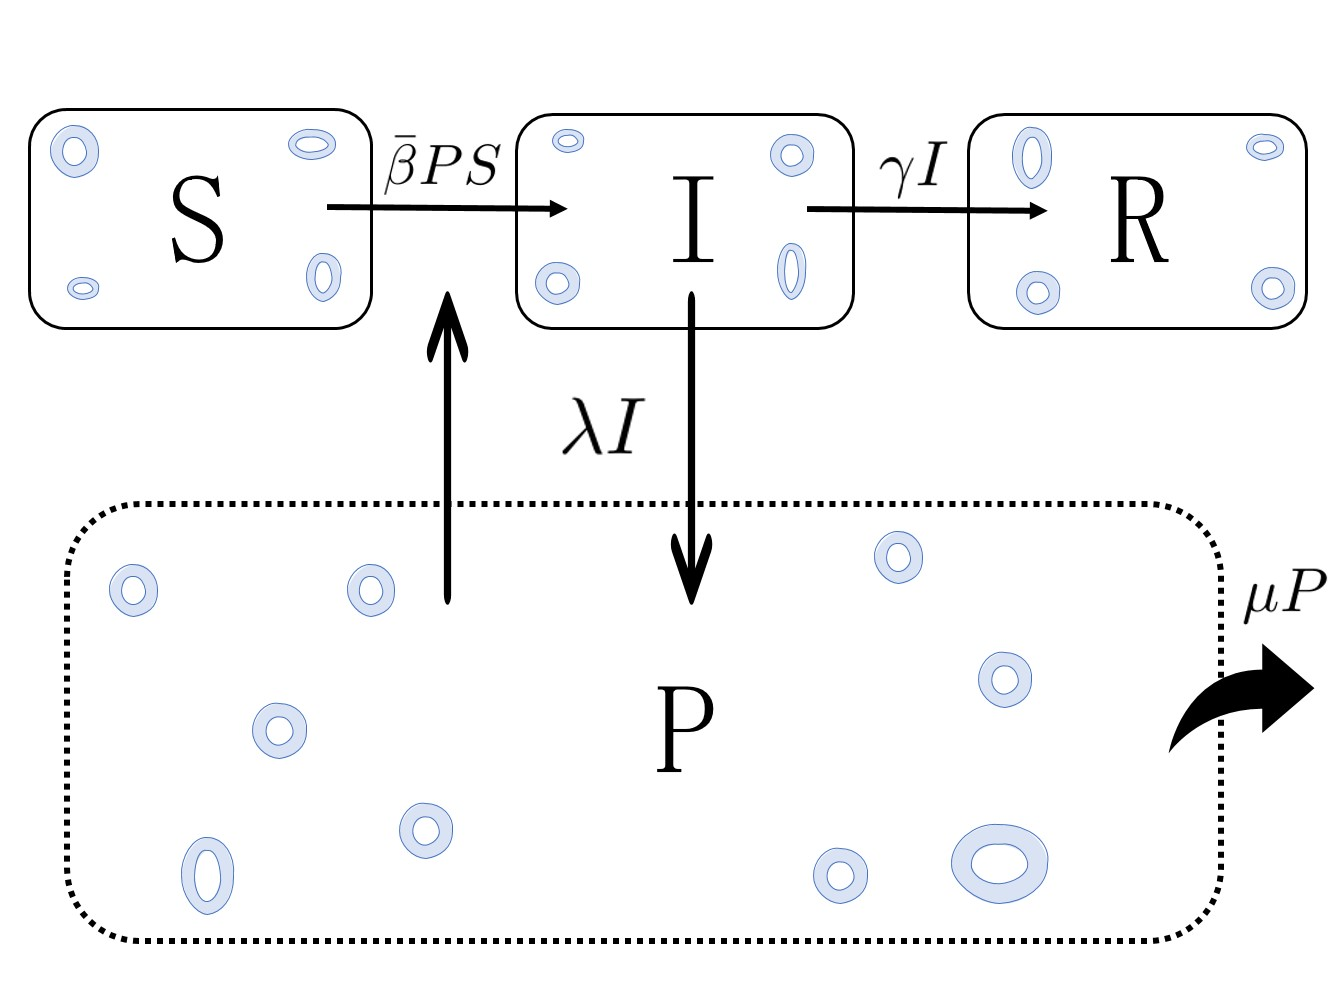
\includegraphics[width=0.8\textwidth]{Figures/SIRP_scheme_mod.jpg}
    \caption[SIRP model flow diagram]{SIRP model flow diagram. The model
        variables are represented
        by capital letters: susceptible hosts ($S$), infected hosts ($I$), dead
        hosts
        ($R$) and the population of parasite ($P$). Arrows represent the
        processes in
        the model with their rates indicated next to them and blue rings
        represent
        parasites. The flow follows the scheme in \cref{eq:scheme_reinfection},
        that
        leads to the system of differential equations in \cref{eq:SIRP}.}
    \label{fig: SIRP_scheme}
\end{figure}

According to the scheme in \cref{fig: SIRP_scheme}, we consider the host in 3
possible states: susceptible, $S$, infected by the parasite, $I$ and removed
(dead), $R$. Then we introduce the parasite population in the medium (water),
$P$. In the model, the $\bar{\beta}$, the disease transmission rate parameter
regulates the infection rate of susceptible hosts and accounts, among other
mechanisms, for the parasite intake rate,
$\gamma$ the mortality of infected hosts, being the inverse of the typical mean
time for an infected host to die; $\lambda$ the production rate of parasites
from infected hosts, and $\mu$ the inverse of the typical life time of the
parasite. $\mu$ can be related to several processes, like biological
deactivation (or survival time) or other general losses, like dilution due to
renewal of water in a closed experiment, natural losses in open ecosystems or
absorption by other filter feeders.
We are not considering the possibility of spontaneous parasite gain, i.e.
immigration, in this version of the model. A summary of the model parameters
can be found in \cref{tab:parameters}.
We do not consider vital dynamics for the hosts, and this implies that the sum
of the $3$ host subpopulations is constant, $N=S+I+R$, as the time scale of the
disease evolution is much faster than the typical life cycle of fan mussels.
The model is similar to the SIP presented in \cite{article_SIP}, except for an
extra term in $\dot{P}$, $-\bar{\beta}PS$, accounting for the fact that when a
parasite infects a host it is absorbed by it. The conditions under which the
SIRP model can be simplified to the SIP model are discussed in
\cref{sec:apprexred}.

In order to build the deterministic model we consider that the population
is large enough to neglect fluctuations and that it is well mixed, so that
spatial effects can be neglected.
In this situation, we consider the infection process to be proportional to
the number of parasites in the medium, so that the average number of contacts
between susceptible fan mussels and the average parasite population is given by
$PS$, and, thus, the change in the number of susceptible fan mussels takes the
form $\dot{S}=-\bar{\beta} PS$,  where the dot over a variable indicates a
differentiation with respect to time: $\dot{S}=dS/dt$.

\begin{table}[H]
    \centering
    \caption{Model parameters description}
    \begin{tabular}{cl:cl}
        \hline \hline
        Variable & Definition             & Parameter & Definition
        \\ \hline
        $S$      & Susceptible host       & $\beta$   & Disease transmission
        rate                                                                 \\
        $I$      & Infected host          & $\gamma$  & Host mortality rate
        \\
        $R$      & Removed host           & $\lambda$ & Production rate of
        parasites by
        infected hosts
        \\
        $P$      & Parasite in the medium & $\mu$     & Parasite
        deactivation/dilution rate
        \\ \hline \hline
    \end{tabular}
    \label{tab:parameters}
\end{table}

Following this argumentation, the scheme in \cref{eq:scheme_reinfection}
and \cref{fig: SIRP_scheme}, one can write the evolution equations of the SIRP
model,
\begin{equation}\label{eq:SIRP}
    \begin{aligned}
        \dot{S} & =-\bar{\beta} P S                    \\
        \dot{I} & =\bar{\beta} P S-\gamma I            \\
        \dot{R} & =\gamma I                            \\
        \dot{P} & =\lambda I-\bar{\beta} P S-\mu P \ .
    \end{aligned}
\end{equation}
Model (\cref{eq:SIRP})	\textit{lives} in the $4$-dimensional (S,I,R,P)
phase space, representing the variables
the populations of individuals in the susceptible, infected and removed
host compartments and of parasites, respectively.

The fixed points of \cref{eq:SIRP} are determined by the
conditions\footnote{We do not consider the trivial fixed point $S=I=R=P=0$ that
    would imply $N=0$ and $P=0$ at all time.}
$I=P=0$, to be fulfilled simultaneously.
We will study the stability of the fixed point defined by $S(0)$,
$I(0)=P(0)=0$ and $R(0)=N-S(0)$.
A linear stability analysis of this fixed point reveals that it has two
null eigenvalues, that stem from the condition $N=S+I+R$ and the conserved
quantity of \cref{app:P_exact}.
The first condition, $S+I+R=N$, implies that it is enough to consider two
of the host populations, e.g. $S$ and $I$, as the third one can be obtained
from the other two. The implications of the conserved quantity reported in
\cref{app:P_exact} are more subtle, as it implies that fixed points are not
isolated, as it happens in ordinary dissipative dynamical systems, and there is
an infinite number (a line of) fixed points for the final state of the
epidemic, depending on the initial conditions. This also implies that the phase
space is foliated by the conserved quantity, $C$ of
\cref{eq:conservedquantity_nacras_I}, and every initial condition, $S_0$, with
a
different value of $C$ leads to a different asymptotic condition, $S_{\infty}$,
just as shown in \cite{Murray_book} for the SIR model (cf. Fig. 10.1 in
\textit{op. cit.}).
The third eigenvalue, that is the largest of the two non-zero eigenvalues,
can be positive if $\beta S_0 \lambda>\gamma(\beta S_0+\mu)$ and negative if
the inequality is reversed, defining the conditional stability of the fixed
point. The fourth eigenvalue is always negative and all the eigenvalues are
always real (\cref{app:linstabfp}).
The instability of the fixed point along the third eigenvalue drives the
beginning of the epidemic.

An extremely important result in epidemiology is the so-called
\textit{basic reproduction number}, $R_0$, a dimensionless number which
represents the number of secondary infections produced by a primary infection
in a fully susceptible population. $R_0=1$ defines the threshold for epidemic
propagation: an epidemic will occur when $R_0>1$, and the number of infected
individuals will grow, at an exponential rate in the early phases of the
epidemic \cite{Castro2020}, while if $R_0<1$ the infection will wane
naturally.
This quantity can be formally obtained making use of the Next Generation
Matrix (NGM) method \cite{Theory_next_gen_matrix, Diekmann2010}. Applying this
formal method to our system of ordinary differential equations (ODE's) one
obtains the following relation for the basic reproduction number
(\cref{app:NGM}),
\begin{equation}\label{eq:R_0_SIRP}
    R_0=\frac{\lambda}{\gamma\parentesi{1+\displaystyle\frac{\mu}{\bar{\beta}
                S(0)}}} \ .
\end{equation}

The threshold condition provided by $R_0$ (\cref{eq:R_0_SIRP}) is
equivalent
to the linear stability condition for the third eigenvalue of the initial,
pre-epidemic, fixed point, as $\bar{\beta} S(0) \lambda>\gamma(\beta S(0)+\mu)$
implies that this eigenvalue is positive and the disease-free equilibrium
state unstable being this
equivalent to $R_0>1$ (\cref{app:linstabfp}).
Thus, if $R_0>1$ the fixed point is unstable, and an epidemic will ensure
if infected hosts, $I$, or parasites, $P$ appear in the system. An epidemic
will propagate until the system reaches an stable fixed point, that signals the
end of the epidemic (\cref{app:linstabfp}).

\subsection{Model reduction} \label{sec:reduction}

The SIRP model lives in a $4$-dimensional phase space and depends on $4$
parameters, what makes difficult to confront it with experimental data. Thus,
we will discuss here
three alternative ways of reducing the model. The first involves an exact
reduction of the model, based on the conserved quantity derived in
\cref{app:P_exact}. The second reduction consists of an approximation to the
previous exact reduction, that turns out to be equivalent to an exact reduction
of a slightly simplified model (without the $-\bar{\beta}SP$ term in the
equation of $\dot{P}$). The third one is based on an approximation valid if the
system parameters fulfil certain conditions.

\subsubsection{Exact reduction of the SIRP model} \label{sec:exactred}

From the conserved quantity derived in \cref{app:P_exact}, it is possible
to write the parasite population in the SIRP model as a function of the host
states as follows,
\begin{equation}\label{eq:P_exact}
    P(S,I)=-\frac{\lambda}{\gamma}\parentesi{S+I} +
    \frac{\mu}{\bar{\beta}}\ln(S) + S + C(0) \ ,
\end{equation}
where $C(0)=P(0)+\displaystyle\frac{\lambda}{\gamma}\parentesi{S(0)+I(0)} -
    \frac{\mu}{\bar{\beta}}\ln(S(0)) - S(0)$.\\

Substituting \cref{eq:P_exact} into the general SIRP model of
\cref{eq:SIRP} we obtain the following nonstandard SIR model,
\begin{equation}\label{eq:SIR_exact}
    \begin{aligned}
        \dot{S} & = \frac{\lambda\bar{\beta}}{\gamma}S\parentesi{S+I} - \mu
        S\ln(S) - \bar{\beta} S^2 - S\bar{\beta} C(0)                        \\
        \dot{I} & = -\frac{\lambda\bar{\beta}}{\gamma}S\parentesi{S+I} + \mu
        S\ln(S) + \bar{\beta} S^2 + S\bar{\beta} C(0) -\gamma I              \\
        \dot{R} & =\gamma I \ .
    \end{aligned}
\end{equation}

Although using the conserved quantity yields an exact reduction from a 4D
dynamical system to a 3D one, the number of independent parameters and initial
conditions remain unchanged, i.e. they still depend on $4$ parameters and $4$
initial conditions. Thus, although useful, (\cref{eq:SIR_exact}) is not ideal
when trying to fit experimental data, and this is the reason for trying a
further approximation to \cref{eq:SIR_exact} to be discussed next.

\subsubsection{Further approximation to the exact reduction}
\label{sec:exactredapp}

A further approximation to \cref{sec:exactred}, that is less restrictive
and expected to be valid in a broader parameter range than the one discussed in
\cref{sec:fastslow} is possible. This approximation reduces the number of free
parameters by one, what is useful in fitting available data.
The approximation consists of neglecting the
$S$ term in \cref{eq:P_exact}, what is possible if $\lambda/\gamma\gg 1$
and also $\mu\ln N/(\bar{\beta} N)\gg 1$, as $S(t)$ decreases monotonically
with time and is, at most, $N$ at the initial time. Interestingly, this
approximation is equivalent to the simplification of the equation for $\dot{P}$
in (\cref{eq:SIRP}) so that the $-\bar{\beta}SP$ is skipped, what yields
exactly
the SIP model of Ref. \cite{article_SIP}. This reduced model has an exact
conserved quantity, $\mathcal{C}$, that differs from that of the SIRP model in
the linear $S$ term (\cref{app:P_exact}).
Using this approximation one can write,
\begin{equation}\label{eq:SIR_exact_reduced}
    \begin{aligned}
        \dot{S} & =\frac{\lambda'}{\gamma}S(S+I)-\mu
        S\ln(S)-S\bar{\mathcal{C}}(0)                 \\
        \dot{I} & =-\frac{\lambda'}{\gamma}S(S+I)+\mu
        S\ln(S)+S\bar{\mathcal{C}}(0)-\gamma I        \\
        \dot{R} & =\gamma I \ ,
    \end{aligned}
\end{equation}
where $\lambda'=\lambda\bar{\beta}$ and $\bar{\mathcal{C}}(0)=\bar{\beta}
    (P(0)+\lambda/\gamma(S(0)+I(0)-\mu/\bar{\beta}\ln S(0)))=\bar{\beta}
    \mathcal{C}(0)$ is a redefinition of the conserved quantity of the SIP
model
\cref{eq:conservedquantitySIP}, $\mathcal{C}(0)$, a constant, such that it
absorbs $\bar{\beta}$ and all initial conditions of the model. The result is
that \cref{eq:SIR_exact_reduced} depends on $3$ parameters and $1$ constant,
compared to \cref{eq:SIR_exact} that depends on $4$ parameters,
facilitating, thus, the use of the model to fit experimental data.

\subsubsection{Model reduction through fast-slow separation}
\label{sec:fastslow}

The third reduction of the $4$-D dynamical model \cref{eq:SIRP} makes the
assumption that the time scale in which the parasite population changes is
faster than the one corresponding to the host. This means that pathogen
deactivation in the medium must be faster than host mortality, which is a very
reasonable assumption. In terms of the rates associated to
each of these processes, this means $\mu>\gamma$. Taking $\mu$ as common factor
in $\dot{P}$ one can write,
\begin{equation}
    \epsilon \dot{P} =\lambda I/\mu-\bar{\beta}SP/\mu-P
\end{equation}
where $\epsilon=1/\mu$ is small, as $\mu$ is large. If furthermore
$\mu\gg\bar{\beta}N$ and  $\lambda\gg \beta P$ one arrives to,
\begin{equation}\label{eq:P_approx}
    P\approx \frac{\lambda}{\mu} I \ .
\end{equation}

Under this approximation the slow subsystem can be written,
\begin{equation}\label{eq:SIRslow}
    \begin{aligned}
        \dot{S} & =-\beta' I S         \\
        \dot{I} & =(\beta' S-\gamma) I \\
        \dot{R} & =\gamma I\ ,
    \end{aligned}
\end{equation}
that is equivalent to the classical SIR model with $\beta'=\bar{\beta}
    \lambda/\mu$ instead of the infection rate $\bar{\beta}$. The reduced $3$-D
model \cref{eq:SIRslow} from the original $4$-D SIRP model \cref{eq:SIRP}
depends on $2$ parameters instead of $4$ as the original model had and $1$
initial condition, e.g. $I(0)=N-S(0)$ if $R(0)=0$, and is much more amenable to
be applied to the analysis of experimental data, as shown in
\cref{sec:validation}.
Furthermore, $\gamma$ could be eliminated through a time rescaling,
$t\rightarrow=t'=\gamma t$ with a redefinition of
$\beta'\rightarrow\beta''=\beta'/\gamma=\beta\lambda/(\mu\gamma)$, leaving the
model as a function of a single effective parameter. However, we will keep both
$\beta'$ and $\gamma$ for convenience when fitting the model to experimental
data in \cref{sec:validation}, as we would need to know anyhow $\gamma$ in
order to analyse the experimental data. The validity of this approximation is
checked numerically in \cref{sec:numericalanalysis}.

\section{Numerical analysis of the model} \label{sec:numericalanalysis}

Due to the impossibility of solving the SIRP model analytically,
in the present section we perform a numerical characterisation of the
model\footnote{All numerical simulations of the dynamical system
    \cref{eq:SIRP} have been carried out using a Runge-Kutta $4$th order
    method,
    with a temporal step $\Delta t=0.001$. Numerically stable results are
    obtain
    with $\Delta t\le 0.01$.}.
Moreover, we show the validity range of the performed approximations to
reduce the SIRP model to an effective SIR model. We start our numerical
analysis by investigating the relative influence of the model parameters on
some epidemiological quantities of interest: the basic reproduction number
($R_0$), related to the existence of an epidemic outbreak, continuing with the
final state of the epidemic, given by the final number of dead individuals
($R(\infty)$) and the maximum of infected individuals ($I_{\textrm{max}}$)
together with the time at which it occurs ($t_{\textrm{max}}$).

In order to identify the most influential parameters of our model
Sensitivity Analysis (SA) will be performed. SA can be divided into two
classes: Local Sensitivity Analysis (LSA) and Global Sensitivity Analysis
(GSA). LSA represents the assessment of the local impact of input factors
variation on model response by concentrating on the sensitivity in the vicinity
of a set of factor values. Such sensitivity is often evaluated through
gradients or partial derivatives of the output functions at these factor
values, such that other input factors are kept constant.
Since epidemic models exhibit a threshold behaviour, controlled by the
dimensionless quantity
$R_0$, it is relevant to study its robustness with respect to small
perturbations by means of the LSA explained above, as its analytical expression
is known.

On the other hand, GSA will be applied to study the influence of the
parameters in the final state of the epidemic and the epidemic peak by
exploring a large domain of the parameter space. In turn, GSA is the process of
apportioning the uncertainty in outputs to the uncertainty in each input factor
over their entire range of interest. A sensitivity analysis is considered to be
global when all the input factors are varied simultaneously and the sensitivity
is evaluated over the entire range of each input factor, in clear contrast to
LSA. Within GSA, first order indices are a measure of the contribution to the
output variance given by the variation of the parameter alone averaged over
variations in other input parameters while second order indices take into
account first order interactions between parameters. While LSA is carried out
analytically (if exact expressions are available), GSA is a purely numerical
approach. Further mathematical details on Sensitivity Analysis can be found in
\cref{app:sensanal}.

For all the sensitivity analysis performed in the following sections, and
in order to avoid ambiguities associated to the definition of $\bar{\beta}$ as
a function of $N$, we assume $N=1$, so that both possible incidences yield
$\bar{\beta}=\beta$ and the numerical results are equivalent.

\subsection{The basic reproduction number $R_0$}

To study the relevance of parameters involved in an epidemic outbreak a LSA
was performed. We analyse the local sensitivity of $R_0$ through the normalised
sensitivity index, so that the function $F(\vec{p})$ of
\cref{eq:sensitivity_analysis} is substituted by the analytical expression of
$R_0$, \cref{eq:R_0_SIRP}.

\cref{fig:Local_Sensitivity_Analysis_R0}(a) shows the sensitivity index for
$R_0$ for specific baseline parameters, where $\lambda$, $\bar{\beta}$ and
$S_0$ contribute to increase the basic reproduction number while $\alpha$,
$\gamma$ and $\mu$ contribute to decrease it, as expected. Moreover, we can see
that $\lambda$ and $\gamma$ are the most influential parameters while $\mu$,
$\bar{\beta}$ and $S_0$ depend on each other. These dependencies cause varying
influences on $R_0$, which are fully depicted in panels
\cref{fig:Local_Sensitivity_Analysis_R0}(b-d). It can be seen that the
influence of $\bar{\beta}$ increases with the increase of $\mu$ and the
decrease of $S_0$. Similarly, the importance of $S_0$ increases with $\mu$ and
decreases with $\bar{\beta}$. On the other hand, the impact of $\mu$ increases
with the decrease of both $S_0$ or $\bar{\beta}$.

\begin{figure}[H]
    \centering
    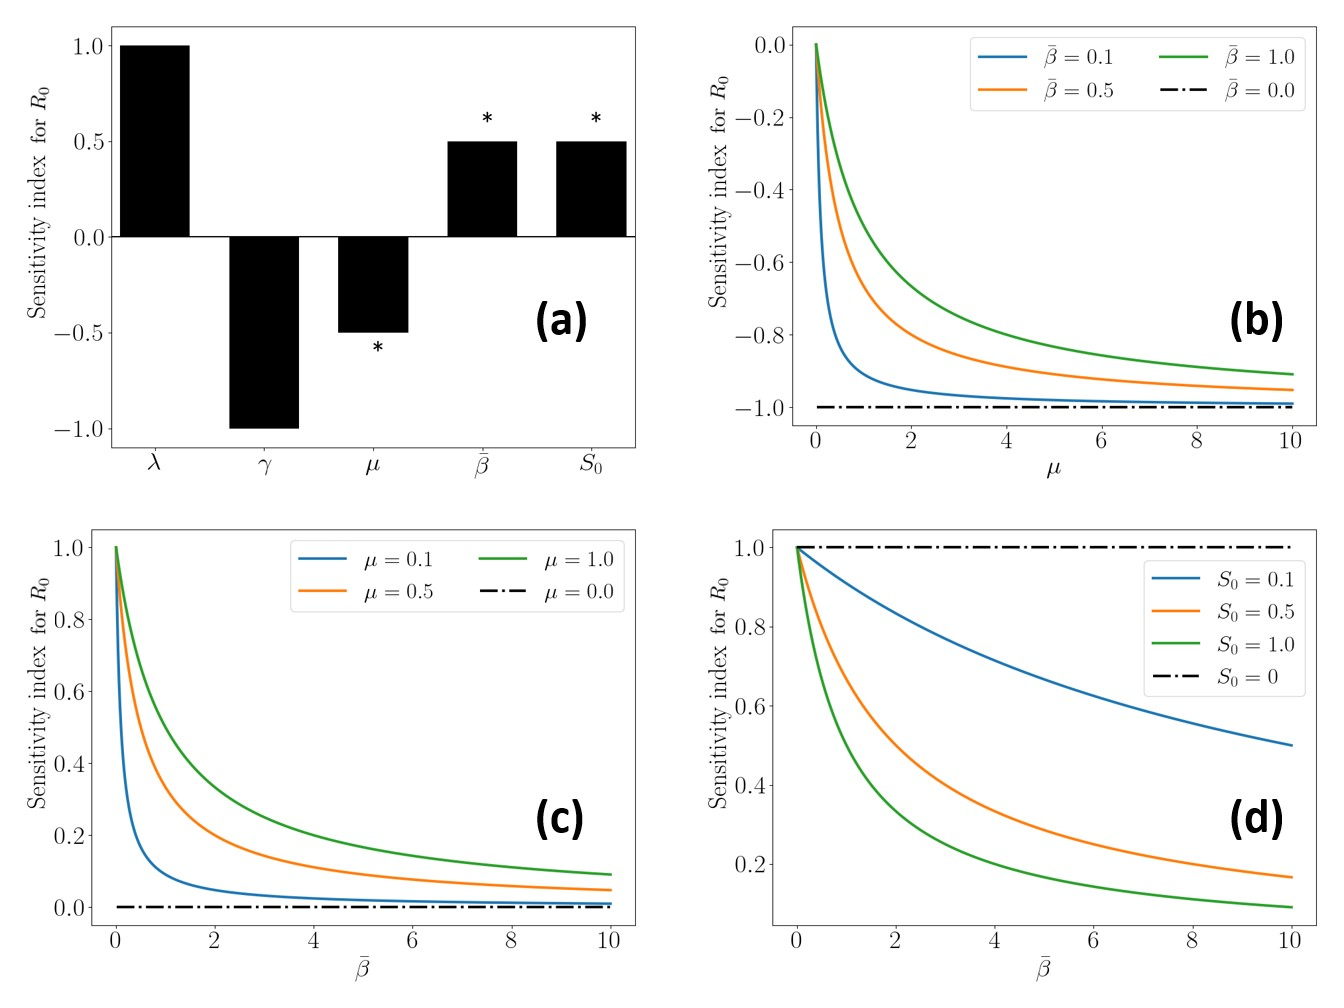
\includegraphics[width=\textwidth]{Figures/R_0_sensitivity.jpg}
    \caption[Sensitivity analysis of $R_0$]{Sensitivity analysis of $R_0$.
        Panel (a): Local sensitivity analysis of $R_0$ for the
        baseline parameters $\lambda=1$, $\gamma=1$ and
        $\mu=\bar{\beta}=S_0=1$. The
        asterisks mark parameters for which the sensitivity index is not
        constant,
        depending on, at least, another parameter. Panels (b-d): Local
        sensitivity
        analysis of $R_0$ with respect to parameters with an asterisk, showing
        the
        different dependence with a second parameter and the effect on the
        varying
        sensitivity index.}
    \label{fig:Local_Sensitivity_Analysis_R0}
\end{figure}

\subsection{Final state of the epidemic}

Another important quantity in epidemiology is the final state of the
epidemic, which can be characterised by the final number of dead individuals,
$R_\infty$. Within our general SIRP model it is not possible to find an
analytical expression for $R(t)$ so that we need to tackle the problem
numerically. To this end, we perform GSA for the final number of dead
individuals in order to determine the most influential parameters for this
quantity. In particular, we apply the Sobol method, discussed in
\cref{app:sensanal}.
The Confidence Interval, CI, obtained in our
study is less than 1\% of the index value, indicating a very high accuracy,
therefore it is not shown in the figures. The results of the explained
procedure are shown in \cref{fig: GSA_R_inf}, where the total order (black),
first order (white) and second order (gray) sensitivity indices for each of the
model parameters are detailed. It can be observed that $\mu$ has a slightly
greater influence than the other parameters with respect to the final number of
dead individuals. Note that the second order indices are larger than the first
order ones for all the parameters, which indicates a high influence of the
nonlinearities in our model, at least for the particular quantity under study.

\begin{figure}[H]
    \centering
    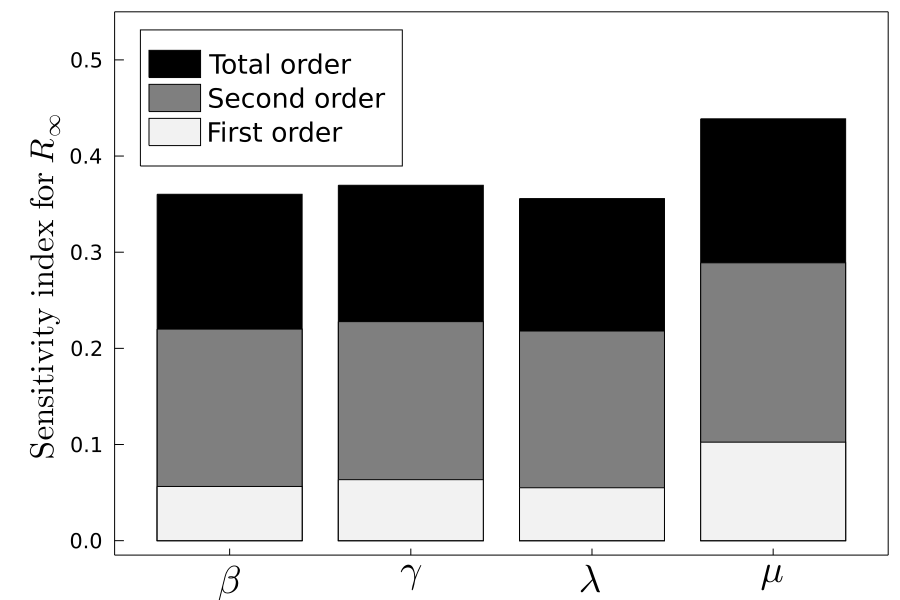
\includegraphics[width=0.7\textwidth]{Figures/GSA_R_inf.png}
    \caption[
        Sensitivity analysis of the final number of dead individuals
        ($R_\infty$)
    ]{Sensitivity indices (LSA) for the final number of dead
        individuals ($R_\infty$) for each one of the indicated parameters. The
        black
        bars represent the total order indices of sensitivity while white
        (grey) colour
        represents the contribution of the first (second) order indices.}
    \label{fig: GSA_R_inf}
\end{figure}

\begin{figure}[H]
    \centering
    \subfigure[Epidemic
        peak]{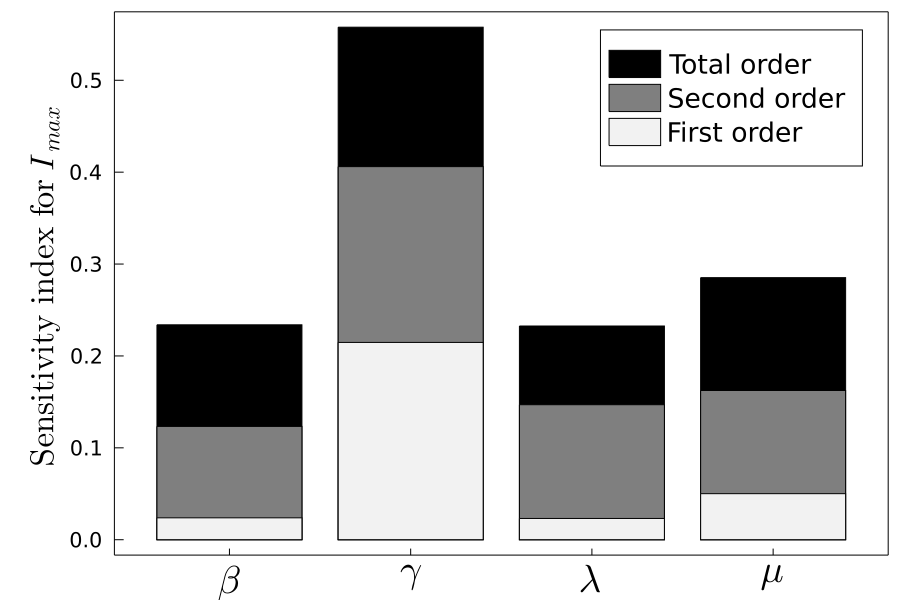
\includegraphics[width=0.49\textwidth]{Figures/GS_peak.png}}
    \subfigure[Time of epidemic
        peak]{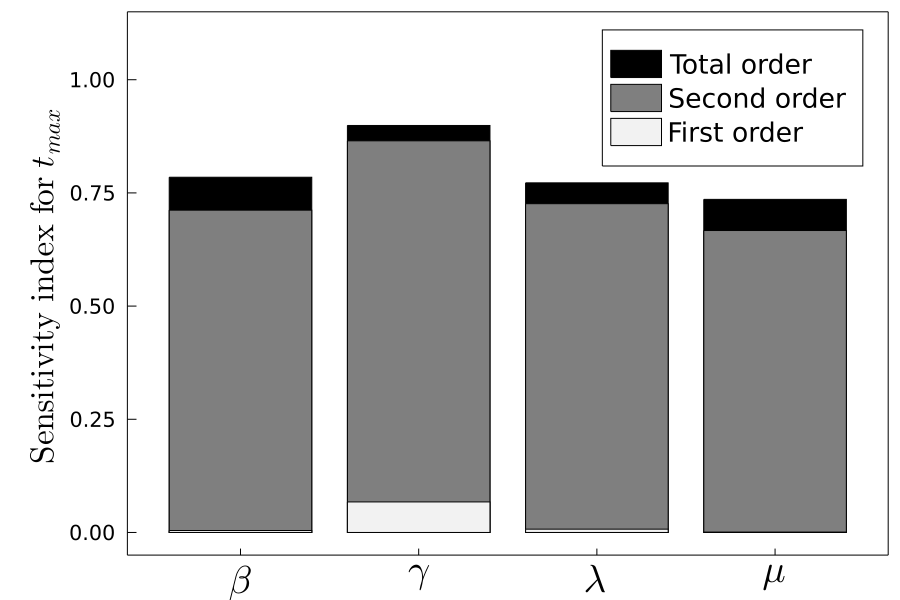
\includegraphics[width=0.49\textwidth]{Figures/GS_peak_time.png}}
    \caption[
        Global sensitivity analysis of the maximum of infected individuals and
        its time occurrence]{Global sensitivity analysis for the maximum of
        infected individuals $I_{\textrm{max}}$ (a) and its time occurrence
        $t_{\textrm{max}}$ (b). The black bars represent sensitivity at all
        orders,  while white (grey) colour represents the contribution of the
        first (second) order indices.}
    \label{fig: GS_analysis}
\end{figure}

\subsection{Maximum of infected individuals}

A GSA of the maximum number of infected individuals, $I_{\textrm{max}}$ and
the time it occurs, $t_{\textrm{max}}$ is performed to study the influence of
the model parameters regarding these quantities. In this case, \cref{fig:
    GS_analysis}, $\gamma$ has greater influence in the epidemic peak than any
of
the other parameters, while for the time at which the peak takes place, all the
parameters have basically the same influence. Again, the second order indices
(the first order interactions between parameters) account for most of parameter
sensitivity, in particular in the time of the epidemic peak, indicating the
high degree of nonlinearity of this effect.

\begin{figure}[H]
    \centering
    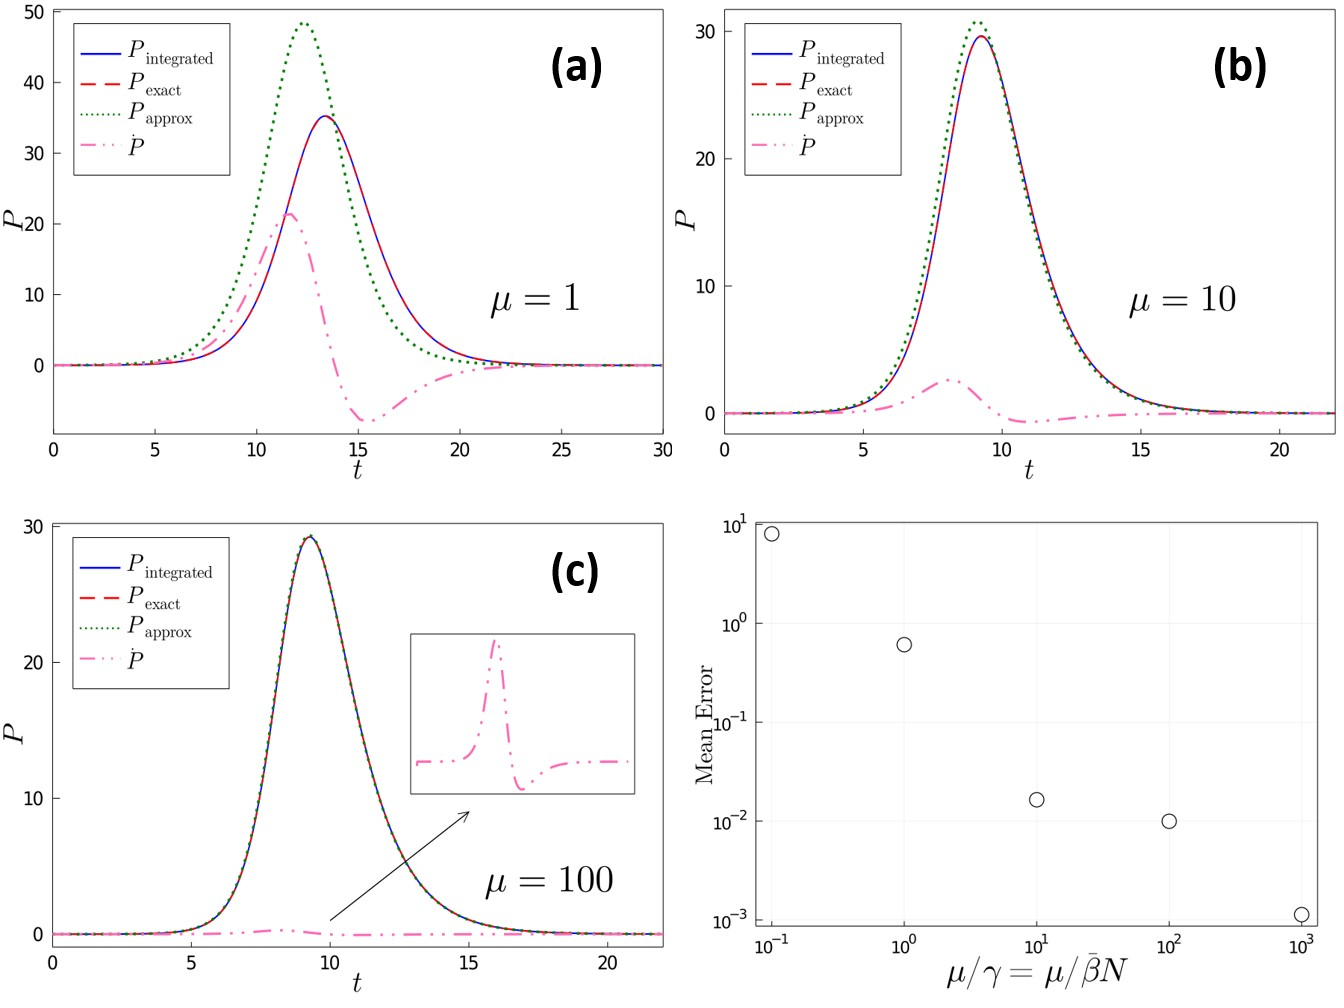
\includegraphics[width=1\textwidth]{Figures/P_comparison.jpg}
    \caption[
        Numerical validation of the timescale approximation for the parasite
        population
    ]{Numerical check of the approximate expression for the pathogen
        concentration, (\cref{eq:P_approx}), $\bar{\beta}=1/50$ and $\gamma=1$:
        (a)
        $\mu=1$; (b) $\mu=10$; (c) $\mu=100$, while $\lambda$ is varied to keep
        $R_0=2.5$, defined in (\cref{eq:R_0_SIRP}) (with $S_0=N=50$), i.e.,
        $\lambda=5,
            27.5, 252.5$ respectively for (a)-(b)-(c), respectively.
        The blue solid line represents the numerically integrated quantity, the
        red dashed line (superimposed to the blue solid one as they are
        identical) is
        the exact solution for this quantity, (\cref{eq:P_exact}) and the green
        dotted
        line accounts for the approximate expression from the timescale
        separation
        (\cref{eq:P_approx}). The dash-dotted pink line represents the
        derivative of
        $P$, $\dot{P}$, in the scaled time frame. Panel (d): Mean error between
        the
        approximate and exact solutions for increasing
        $\mu/\gamma=\mu/\bar{\beta}$.}
    \label{fig:P_comparison}
\end{figure}

\subsection{Numerical verification of the fast-slow approximation}

The parasite concentration approximation, based on a timescale separation
discussed in \cref{sec:fastslow}, is now verified by computational means. The
verification was performed using both mass action and standard incidence, but
for the sake of simplicity we show only the results for the standard incidence
case. Worth is to say that, mathematically, changing from standard incidence to
mass action involves only a rescaling of the $\bar{\beta}$ parameter, so that
the numerical results are exactly the same. \cref{fig:P_comparison} contains a
comparison for $3$ different values of the parasite deactivation rate, $\mu$.
It can be seen that the approximation is poor when $\mu\sim
    \gamma,\bar{\beta}N$ \cref{fig:P_comparison}(a), as it could be expected.
On
the other hand, the approximation is quite good when $\mu$ is one order of
magnitude larger than $\gamma$ and $\bar{\beta}N$ \cref{fig:P_comparison}(b),
while it is extremely accurate when $\mu$ is two orders of magnitude larger
than $\gamma,\bar{\beta}N$, \cref{fig:P_comparison}(c). The figure also shows
the numerical value of $\dot{P}$ (pink dashdot), and it can be checked how it
becomes smaller as $\mu$ increases compared to $\gamma,\bar{\beta}N$,
justifying the timescale separation of \cref{sec:fastslow}. Finally,
\cref{fig:P_comparison}(a-c) also shows (dashed red line) the analytical value
for $P(S,I)$ derived in \cref{eq:PSI_exact}, that matches perfectly the result
of the numerical integration of \cref{eq:SIRP}, as should be the case.

\begin{figure}[H]
    \centering
    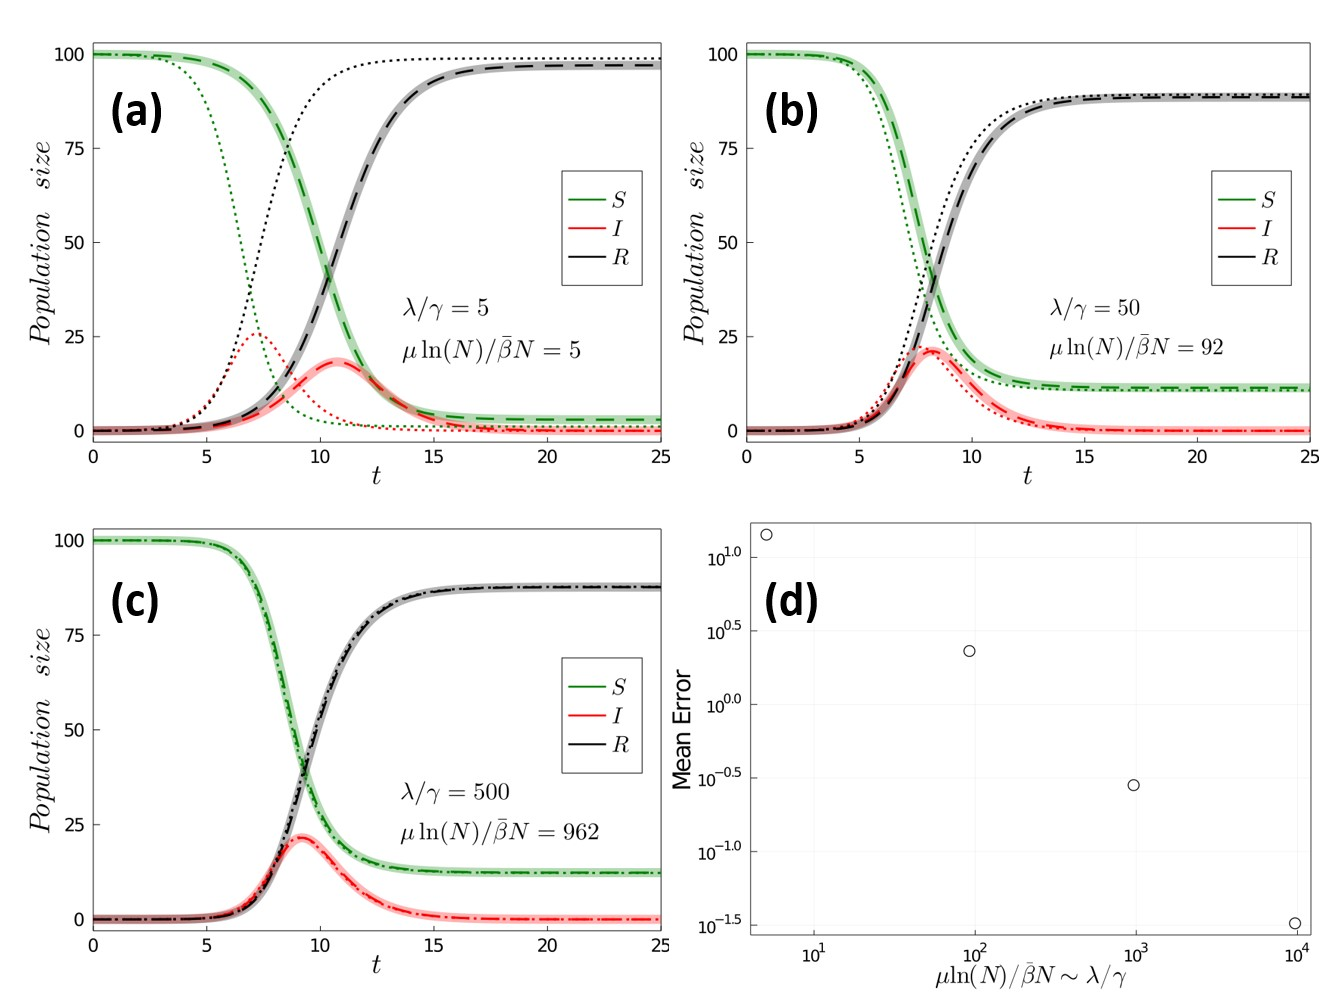
\includegraphics[width=1\textwidth]{Figures/exact_reduction_approx.jpg}
    \caption[
        Numerical verification of the exact model reduction and the subsequent
        approximation
    ]{Numerical check of the exact model reduction along with the
        subsequent approximation shown in \cref{sec:exactred} with $N=100$,
        $\bar{\beta}=1/100$, $\gamma=1$, (a) $\lambda=5$, $\mu=1.1$; (b)
        $\lambda=50$,
        $\mu=20$; (c) $\lambda=500$, $\mu=209$. $R_0=2.38$ for all the panels.
        The
        solid semitransparent lines represent the original 4D model, the dashed
        lines
        the exact reduction and the dotted lines the approximate model from the
        exact
        reduction. Panel (d): Mean error between the approximate and exact
        solutions
        for increasing $\mu\ln(N)/\bar{\beta}N$ and $\lambda/\gamma$ while
        $R_0=2.38$
        is kept constant.}
    \label{fig:verification_exact_reduction}
\end{figure}

\subsection{Numerical verification of the model approximation from the
    exact reduction} \label{sec:apprexred}

The numerical verification was performed for both mass action and standard
incidence, but for the sake of simplicity in
\cref{fig:verification_exact_reduction} we show only the results for the
standard incidence case. First, and as it should be because it is an exact
result, the exact reduction of the SIRP model discussed in \cref{sec:exactred}
matches perfectly the numerical results obtained from the full model for all
possible parameter values,
\cref{fig:verification_exact_reduction}(a-c).
Regarding the approximation to the exact reduction, one can see
how the approximation converges to the exact solution as the parameters
fulfil the conditions indicated in \cref{sec:exactredapp}, namely that both
$\gamma/\lambda\gg 1$ and $\mu\log(N)/\bar{\beta N}\gg 1$, becoming very
accurate if these ratios are larger than $1$ by two orders of magnitude or more
(\cref{fig:verification_exact_reduction}(c)). We recall that in this case
the SIRP model converges to the SIP model of \cite{article_SIP}. Conversely,
the approximation is poor when any of these two ratios is of order $1$
(\cref{fig:verification_exact_reduction}(a)), while
\cref{fig:verification_exact_reduction}(b) presents the result in an
intermediate case, in which the approximation is fair.

\section{Model validation with data of the \textit{Pinna nobilis} Mass
  Mortality Event}
\label{sec:validation}

In this section, the general SIRP model is validated against collected data
from the \textit{Pinna nobilis} Mass Mortality Event. As explained in
\cref{sec:Introduction_Nacras_I}, the disease is caused by the parasite
\textit{Haplosporidium pinnae} and the hosts, \textit{P. nobilis}, are sessile
bivalves endemic of the Mediterranean Sea. Thus, this epidemic is a perfect
candidate to be described by the SIRP model. In the model, parasite production
occurs only inside infected hosts, and parasites are released to the medium,
either through their respiratory or digestive system. The simultaneous
occurrence of the different possible stages of the parasite (uni- and
bi-nucleate cells, multinucleate plasmodia, sporocysts and uninucleate spores)
in the same host individual is not common among haplosporidans and makes
\textit{H. pinnae}  different from previously known haplosporidan species
\cite{CATANESE20189}. The occurrence of uni- and binucleate stages suggest
possible direct transmission from infected to healthy fan mussels, as observed
in \textit{B. ostreae} and \textit{B. exitiosa} \cite{hine1996ecology,
    Culloty2007, Audemard2014}. Additionally, the presence of spores (a
dormant,
resistant stage) could allow long persistence in the environment and the
hypothetical involvement of an intermediate host as suggested for \textit{H.
    nelsoni} and \textit{H. costale} \cite{Andrews1984,
    haskin1988uncertainties,
    powell1999modeling}. While uninucleate cells are always detected in
infected
fan mussels, sporulation has been only detected sporadically
\cite{CATANESE20189}. Thus, we assume that infection occurs mostly through
uninucleate (or binucleate) cells by direct transmission (as the experimental
observations in captivity point out, see \cite{March}).
We do not consider disease transmission through other stages. We do not
consider spores, given the infrequent observation of spores and the current
lack of experimental information about spore transmission (that could involve
another intermediate host species). Regarding plasmodia and sporocyst stages,
these stages are too large to be released through the epithelium. The
distinction between uninucleate and binucleate cells seems unnecessary at this
level of representation, as these phases only participate in parasite
proliferation inside infected hosts, a process that we consider in an effective
way. Finally, the evidence of the time course of the disease compared to the
long life cycle of {\it P. nobilis\/} suggests host vital dynamics (i.e.
recruitment (reproduction) and natural death) can be neglected.

After an epidemic outbreak that took place in Portlligat, in the north east
of Catalonia, $215$ \textit{Pinna nobilis} individuals were extracted from
their natural medium in order to be preserved as a genetic reserve in several
controlled water tanks of different institutions in Spain \cite{March}. The
institutions that participated in this preservation effort were IFAPA, IEO,
IRTA, IMEDMAR-UCV and Oceanogr\`afic of Valencia. The original idea was to
rescue the individuals before infection, however, the subsequent evolution of
the rescued \textit{Pinna nobilis} populations indicates that some individuals
were already infected at the time of extraction (and/or in contact with some
amount of the parasite transferred from sea water).
This allowed the opportunity to use the data of the time evolution of the
epidemic in the controlled water tanks, reported in \cite{March}, to evaluate
the described SIRP model\footnote{Data use in this work with the purpose of
    validating and fitting parameters for the SIRP model have been taken from
    the
    Supplementary Information of \cite{March}}. The empirical data consists of
the
proportion of survivors as a function of time in the controlled water tanks
with a temporal resolution of one month. Despite the fact that the temperature
of the water in the tanks was controlled, it was sharply lowered in most of the
tanks when mortality started to appear within the population, as a last effort
to keep the rest of the population safe and alive, since keeping the
temperature below  approximately $13.5\, {}^o$C is a known strategy to preserve
\textit{Pinna nobilis} individuals as disease expression is minimal
\cite{Cabanellas2019}. Fortunately, two of the tanks kept its temperature
approximately constant during the full recorded time. This is the case of the
tanks in IFAPA in Huelva and the Oceanogr\`afic of Valencia (OCE), both Spanish
institutes. These water tanks have been selected to validate our model,
maintaining constant temperatures of $14\, {}^o$C and $17\, {}^o$C,
respectively.

First we will fit the exact reduction of the SIRP model, assuming
$\mu\log(N)\gg\bar{\beta}N$ and $\lambda/\gamma\gg 1$ as discussed in
\cref{sec:exactredapp}, namely \cref{eq:SIR_exact_reduced}.
This reduced model depends on three parameters ($\lambda'$, $\mu$,
$\gamma$) and one constant, $\bar{\mathcal{C}}(0)$ (see
\cref{sec:exactredapp}), that is related to the initial conditions of the
model. The order of magnitude
of the mortality rate can be deduced from data, with an estimated value of
$\gamma\approx\SI{1}{month^{-1}}$. We fix this parameter in order to give some
biological information to our model prior to the computational fit. We focus on
the $R$ compartment, as it can be retrieved directly from data in
\cite{March}\footnote{The number of dead individuals can be obtained as
    $R=N-S$, where $S$ is the population of survivors and $N$ is the total
    number
    of individuals in the tanks,
    $50$ (IFAPA) and $5$ (Oceanogr\`afic), respectively}.
We use a box-constrained variant\footnote{We constrain the optimisation
    because the unconstrained optimisation to the full range of the parameters,
    i.e, from $0$ to $\infty$ is not practical.} of the well known BFGS
optimisation algorithm \cite{BFGS} with a common $\textrm{L}2$ loss function,
also known as Residual Sum of Squares (RSS)\footnote{The algorithm is
    implemented within the Julia high-level programming language \cite{julia}
    using the DifferentialEquations.jl package
    \cite{DifferentialEquations.jl}.}.
By running this algorithm one observes that the optimal parameters tend to be
the ones in the boundary of the box-constrained parameter space.
Furthermore, if the box size is increased (or decreased) the optimal
parameters continue to be in the boundary of the box-constrained parameter
space.
This indicates that there exist several parameter combinations that
optimally fit the data, and the combination parameters found by the
optimisation algorithm are only marginally optimal with respect to other
parameter values. The locus (actually a valley) of marginal optimal parameters
can be seen in the right hand side panels of \cref{fig: exact_SIR_fit}, where
the cost function value of the optimisation algorithm is plotted as heat map.

\begin{figure}[H]
    \centering
    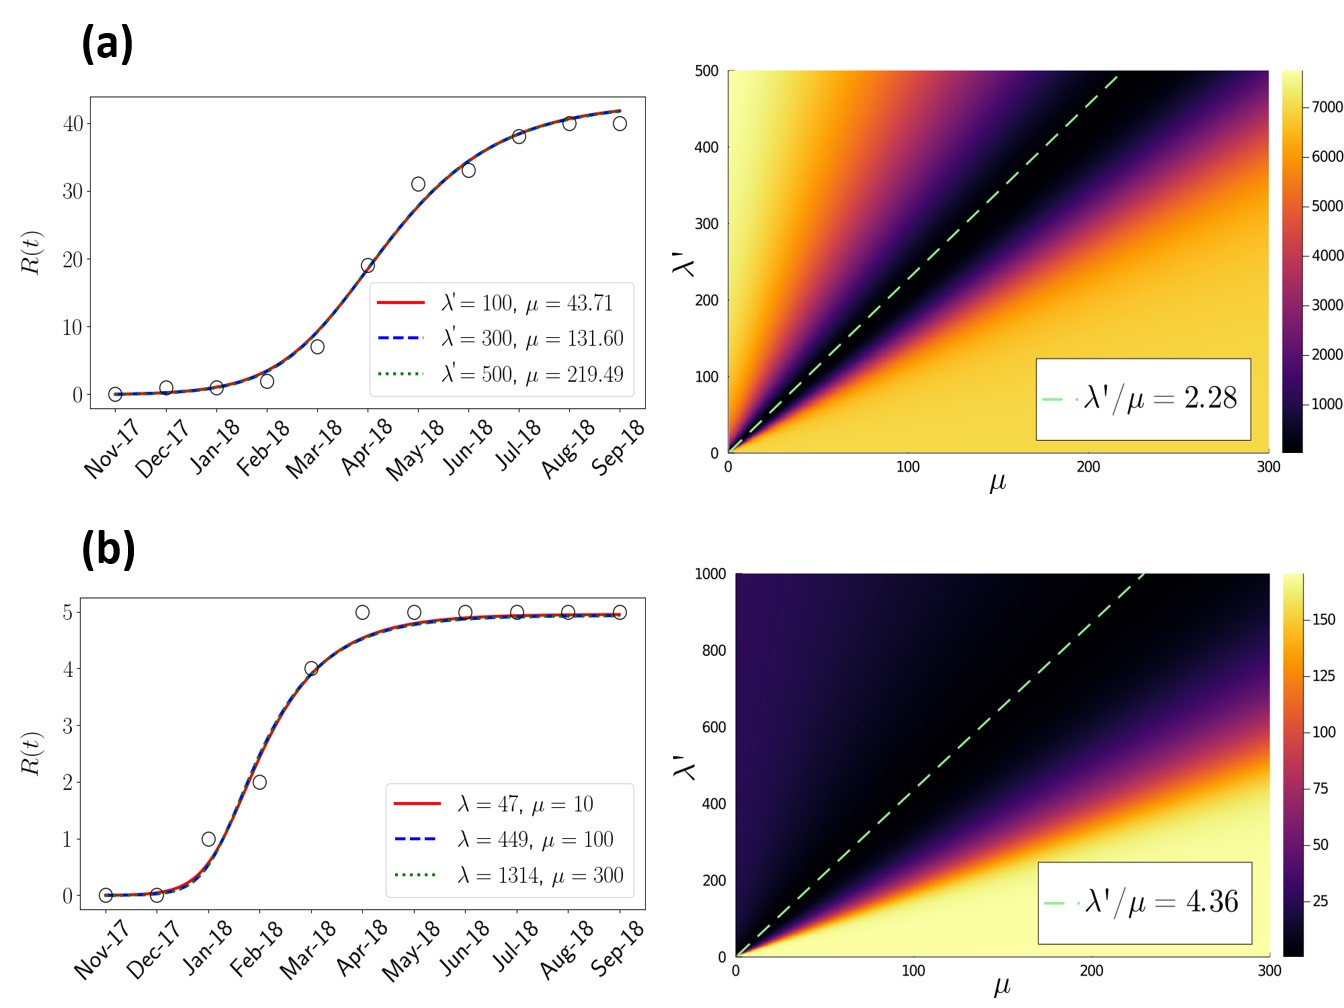
\includegraphics[width=1\textwidth]{Figures/exact_SIR_fitting.jpg}
    \caption[
        Parameter estimation of the exact reduction of the SIRP model
    ]{Parameter estimation for the approximation from the exact
        reduction of the SIRP model (\cref{eq:SIR_exact_reduced}) using data
        from IFAPA
        (panel (a)) and OCE (panel (b)) water tanks, at $\SI{14}{\degree C}$
        and
        $\SI{17}{\degree C}$ respectively. Left panels represent several fits
        of the
        model to empirical data of the number of dead hosts ($R(t)$) using
        different
        optimal combinations of the parameters. Right panels are the RSS
        errors as a
        function of the input parameters, where the green dashed line
        represents the
        set of optimal combinations of the parameters with $RSS=60, 0.8$ for
        IFAPA and
        OCE, respectively.}
    \label{fig: exact_SIR_fit}
\end{figure}

Now we reach the point regarding the dilemma between mass action and
standard incidence discussed in \cref{subsec:modtruct}. If one does not correct
the $\bar{\beta}$ parameter with the size of the host population, $N$, that is
equivalent to assuming the mass action incidence $\bar{\beta}=\beta$, the
values that one would obtain for $\beta'=\beta\lambda/\mu=\lambda'/\mu$ for
both populations take disparate values in both tanks: $\beta'=0.046$ for the
IFAPA data set and $\beta'=0.87$ for the Oceanogràfic (OCE) data set, a factor
of $19$ between them while their temperatures differ only by $3\,{}^o$C.
These numbers indicate that the standard incidence is more reasonable, what
amounts to choosing $\bar{\beta}=\beta/N$, where the final values of the
reported parameter $\beta'$ should be multiplied by $N=50$ for the IFAPA tank
and $N=5$ for the OCE tank. The final result is then $\beta'=2.28$ and
$\beta'=4.36$ for IFAPA and OCE tanks, that are the values reported in
\cref{fig: exact_SIR_fit}, implying that an almost twofold increase of the
$\beta'$ parameter corresponds to an increase of $3\,{}^o$C. This relation is
in good agreement with the typical changes in rates of a wide range of
organisms with a $\SI{3}{\degree C}$ change in temperature, while a 19-fold
change in the rate would imply at least a $\SI{30}{\degree C}$ change in
temperature (\cref{app:rate_change}).

\begin{figure}[H]
    \centering
    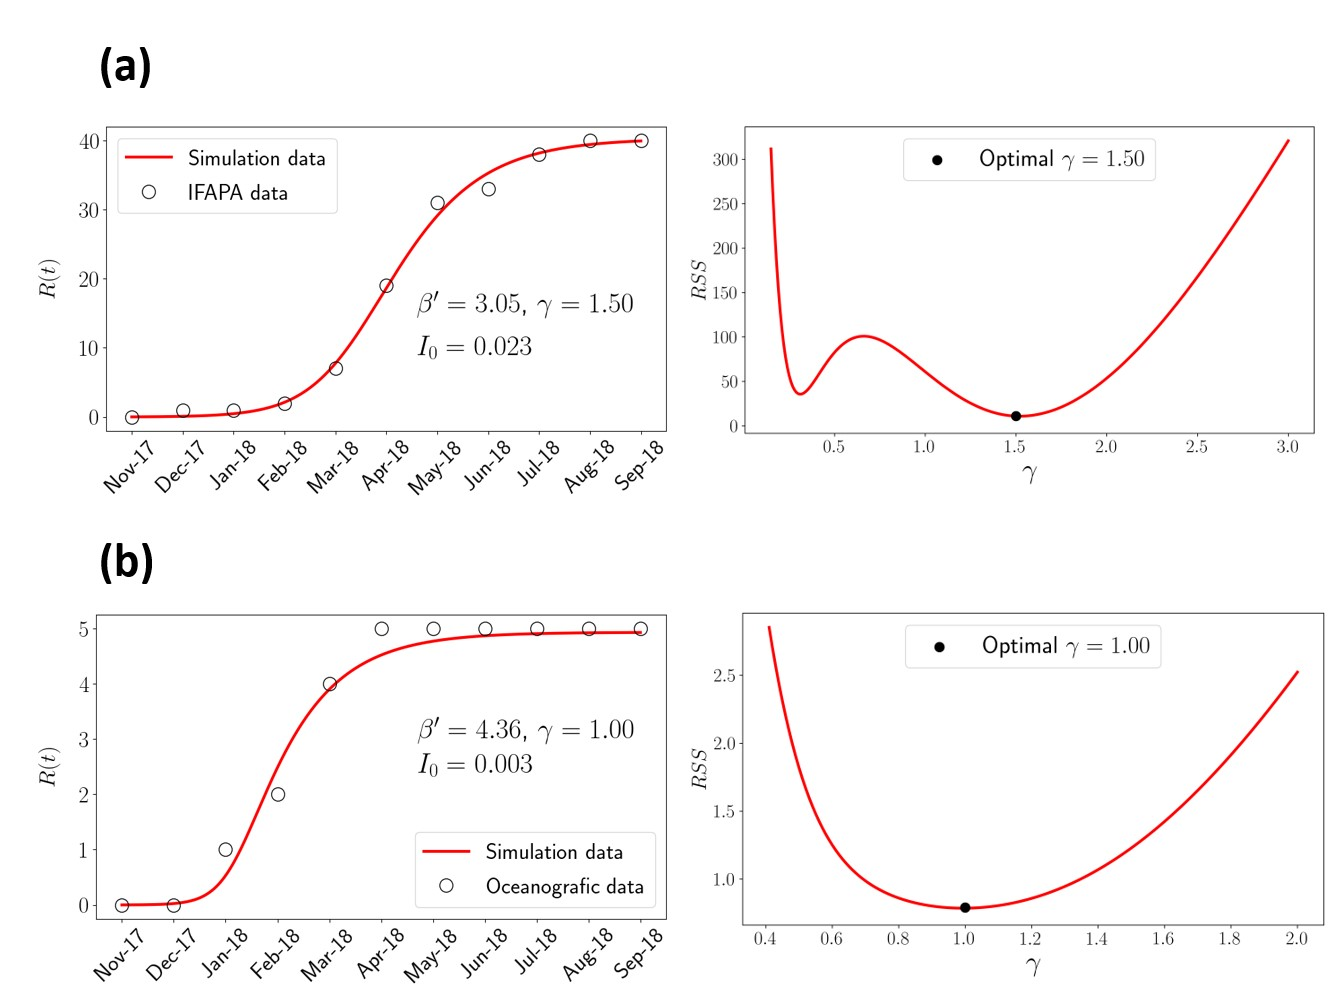
\includegraphics[width=1\textwidth]{Figures/approx_SIR_fitting.jpg}
    \caption[
        Parameter estimation of the approximate SIR model
    ]{Parameter fitting for the R compartment to model
        (\cref{eq:SIRslow}) using data from IFAPA (panel (a)) and Oceanogràfic
        (panel
        (b)). The left part of both panels of the figure shows the optimal fit
        of the
        model to empirical data with $RSS=10.9, 0.8$ for IFAPA and OCE,
        respectively.
        The right panels show the variation of the $RSS$ error for some values
        of
        $\gamma$.  The $\beta'$ values have been obtained assuming a standard
        incidence, as explained in the main text.}
    \label{fig:approx_SIR_fit}
\end{figure}

The fact that there is an infinite number of combinations of the parameters
that optimally fit the real data suggests that, as two parameters are slaved
one to each other, that the model
admits a further reduction. This reduction corresponds exactly to the
approximate $SIR$ model derived in \cref{eq:SIRslow}, with the relationship
$\beta'=\lambda'/\mu$, as anticipated. So, this gives further corroboration to
the use of the $SIR$ model \cref{eq:SIRslow} to fit $\beta'$ as the free
parameter (fixing the value of $\gamma$ and with $I_0$ as the initial condition
determined by the fit). For consistency with the previous fitting we expect to
obtain $\beta'=2.28$ and $4.36$ as the optimal parameters for the IFAPA and OCE
water tanks, respectively, and this is the case.

Interestingly, as reduced model \cref{eq:SIRslow} has fewer parameters to
fit we can relax our initial assumption of $\gamma=\SI{1}{month^{-1}}$ and
check how the fit improves or worsens when varying $\gamma$.
In \cref{fig:approx_SIR_fit} a fit of the reduced SIR model
\cref{eq:SIRslow} is shown for the IFAPA (top) and Oceanogràfic (bottom)
controlled water tanks\footnote{The $N$ correction corresponding to standard
    incidence has already been applied to these values.}.
\cref{fig:approx_SIR_fit}(c-d) shows the $RSS$ error as $\gamma$ is varied.
It can be seen that for the IFAPA water tanks $\gamma=\SI{1.5}{month^{-1}}$
yields more accurate results, while for the Oceanogràfic water tanks
$\gamma=\SI{1}{month^{-1}}$ remains optimum. This shows a decrease in the mean
removal time $1/\gamma$ for lower water temperatures, with the finite size
errors inherent to the OCE tank (as $N=5$).
In the left panels the simulated curve of dead individuals, $R$
compartment, as a function of time for the optimal fitted parameters is
confronted to the experimental data, showing a remarkable agreement. With the
optimum values of $\gamma$, in the IFAPA tank (now with
$\gamma=\SI{1.5}{month^{-1}}$) a new value of $\beta'=3.05$ is obtained,
implying a probably more reasonable ratio of $1.43$ for $\beta'$ in both tanks
(it was $1.91$ in the original fit).
From the optimal parameters we obtain the basic reproduction number, since
$R_0=\beta'/\gamma$ we have that $R_0^{\textrm{IFAPA}}\simeq2$ and
$R_0^{\textrm{OCE}}\simeq4$, clearly above the epidemic threshold.

Summarising, the SIRP model is able to fit two sets of experimental data,
agreeing with a standard incidence, according to which the infection rate
depends on the amount of parasites per pen shell individual. \textit{Pinna
    nobilis} individuals in
the IFAPA experiment were actually distributed in $4$ tanks, and the
standard incidence is compatible with this experimental aspect. The temperature
dependence of the fitted parameters in this range ($14-17 {}^o C$, appears to
be compatible (although experiments at different temperatures would be needed)
with an Arrhenius dependence of the infection parameters, also known as
Boltzmann-Arrhenius
\cite{Brown2004,Molnar2017}, that can be extended to account for the
expect unimodal dependence on temperature, with a maximum infectivity at a
characteristic temperature for the parasite \cite{Molnar2017}. Therefore, we
can assume that global change (or temperature shifts) is expected to have
complex effects on infectious diseases, causing some to increase, others to
decrease, and many to shift their distributions \cite{Rohr2020}.
In the particular case of pen shell mortality, our model results suggest the
proposed mechanism of lower disease expression at lower temperatures. This
might have direct consequences for the development of the mortality event and
offers a bleak perspective for the future and specifically in the eastern
Mediterranean basin, where the mortality was observed later due to current
patterns but average temperatures tend to be higher than in the western part of
the Mediterranean.

\section{Conclusions} \label{sec:conclusions}

In this work we have analysed a compartmental model to study marine epizootics
for sessile hosts assuming infection by direct transmission through waterborne
parasites. Moreover, we have used data from the recent mass mortality event of
\textit{Pinna Nobilis} in the Mediterranean Sea as a case study to validate our
model. Compartmental models are routinely used in the study of disease
infection and propagation in terrestrial ecosystems, including the study of the
current Covid-19 pandemic (see, e.g., \cite{Castro2020}). However, these
models are starting to be used only recently in the study of marine epizootics
\cite{article_SIP}, while proliferation models have been the most popular in
the field \cite{Powell2015}. A reason for
the low popularity of compartment models in the study of marine epizootics is
that there are some aspects in its modelling that differ from the now standard
application to terrestrial ecosystems \cite{MCCALLUM_intro}. An important
difference is that, in principle, (micro)parasites need to be modelled
explicitly in marine ecosystems, while often they are not included in the
description in terrestrial ecosystems  \cite{May1979}.

The SIRP model has $4$ compartments and depends on $4$ parameters, so that it
is not quite amenable to theoretical analysis. At the same time, due to the
large number of parameters of the model, using it to analyse experimental
observations can be cumbersome in practice if the parameter values are unknown.
Nevertheless, we have shown three reductions of the model, one exact and two
approximate ones, that can be useful to overcome these limitations that are
typically present at the first stages of emergent epidemics. Indeed, the
timescale approximation is able to fit the collected data of our case study for
some optimal parameters, as shown in \cref{sec:validation}. This approximation
is particularly useful as it only depends on $2$ parameters, the death rate of
infected hosts, $\gamma$ and an effective infection rate, $\beta'$. Although
this approximation simplifies the fitting procedure, there is a price to be
paid in this analysis. The infection parameter, $\beta$, and the parameters
regulating proliferation, $\lambda$, and deactivation/dilution of the parasite,
$\mu$, become entrained into a single effective parameter, $\beta'$. Thus, the
full understanding of the different effects at play in the system requires
further work. Furthermore, we have shown that an epidemic model for immobile
hosts can be reduced to the standard SIR model, which assumes direct contact
among the hosts, i.e. that the hosts are mobile. This reduction is only valid
when the time scale of the parasites is much faster than that of the hosts,
i.e. $\mu\gg\beta N,\gamma$. Thus, our work provides a ground to apply the SIR
model in marine epidemics of sessile hosts that fulfil the required conditions.

In a world with many possible new epizootics, we believe that our reduced model
can be specifically useful to understand key features of those emerging
diseases characterised by the spreading of waterborne parasites in a relatively
fast way, provided that the temporal evolution of the disease can be determined
for, at least, some set of individuals. Thus, some of the key parameters can be
fitted to the available experimental data as shown in \cref{{sec:validation}}.
Still, the fitted relevant parameters may need to be supplemented with further
information or targeted experiments. We hope that this approach can be useful
in understanding emerging diseases in shellfish species of economic not only
ecological value, and also, with suitable modifications, in aquaculture. It is
noteworthy that our case study is a haplosporidan waterborne parasite.	In
fact, waterborne haplosporidans have been responsible for some of the most
significant and consequential marine disease epizootics on record and are
considered the major pathogens of concern for aquatic animal health shellfish
industries around the world \cite{Arzul2015}. The SIRP model is the simplest
model that one could think of having in mind its practical application, but
could be extended to incorporate further effects that are so far described in
an effective way.